\documentclass{article}
%Required: You must have these
\usepackage{Sweave}
\usepackage{graphicx}
\usepackage{tabularx}
\usepackage{hyperref}
\usepackage{natbib}
\usepackage{pdflscape}
\usepackage{array}
\usepackage{gensymb}
%\usepackage[backend=bibtex]{biblatex}
%Strongly recommended
  %put your figures in one place
%\SweaveOpts{prefix.string=figures/, eps=FALSE} 
%you'll want these for pretty captioning
\usepackage[small]{caption}

\setkeys{Gin}{width=0.8\textwidth}  %make the figs 50 perc textwidth
\setlength{\captionmargin}{30pt}
\setlength{\abovecaptionskip}{10pt}
\setlength{\belowcaptionskip}{10pt}
%Optional: I like to muck with my margins and spacing in ways that LaTeX frowns on
%Here's how to do that
 \topmargin -1.5cm        
 \oddsidemargin -0.04cm   
 \evensidemargin -0.04cm  % same as oddsidemargin but for left-hand pages
 \textwidth 16.59cm
 \textheight 21.94cm 

\begin{document}
\bibliographystyle{/Users/ailene.ettinger/Documents/GitHub/fishphen/refs/bibstyles/amnat.bst}% i moved a style file into the ospree git repo. feel free to add whatever style you like and update, lizzie! I don't have besjournals

\Sconcordance{concordance:orcaphen.tex:orcaphen.Rnw:%
1 98 1}


\title{Shifts in Orca Phenology and their Prey in the Salish Sea}
\date{\today}
\maketitle

\section* {Background}
\begin{enumerate}
\item Southern resident killer whales (SRKWs) are a threatened population, recieved much scientific and public attention.
\item  SRKWs use of the Salish Sea varies seasonally across two broad areas: the upper Salish Sea 
(north of Admiralty Inlet, reference Map).
\item Efforts are underway to alter hatchery production to benefit orca whales, because one of the threats facing SRKWs is thought to be lack of prey. We know that SRKWs forage on chinook salmon as a primary food source (cite hanson papers), but there are lots of questions about what other species they use and how their prey varies seasonally. 
\item SRKW activity is generally thought to be related to finding prey. In recent decades, salmon abundance and phenology has shifted in the Salish Sea \citep{weinheimer2017,reed2011,ford2006}(add Nelson for chinook hatchery release timing, others for abundance data), though rates vary by species and location. We would therefore expect SRKW phenology to have shifted during this time, if prey is a primary driver of their activity in the Salish Sea. 

\item SRKWs may be spending more time in Puget Sound \citep{olson2018}. However, the details are unclear because monitoring effort has also increased duiring this time. Understanding how SRKW activity varies seasonally and how these seasonal patterns have shifted in recent decades will allow us to develop and test hypotheses about potential drivers of these shifts, which in turn will provide information that may be useful for management decision-making to conserve SRKWs.
\item Additionally: could make this more explicitly about changes in effort/presence-only database and citizen science. 
\end{enumerate}
\section* {Research Questions}
Here, we ask:
\begin{enumerate}
\item Has the timing of SRKW activity (phenology) shifted in the upper Salish Sea and/or Puget Sound? (First observation date, Last observation date, number of days observed)
\item If there have been phenological shifts in SRKW activity, do these shifts coincide with shifts in phenology or abundance of their prey (chinook, coho, chum salmon)?
\end{enumerate}


\section* {Methods}
\begin{enumerate}
\item Data
\begin{enumerate}
\item To quantify orca seasonal phenology over time, we used the OrcaMaster Database for Whale Sighting Data (Whale Museum), which includes data from five main sources, including public sightings networks (e.g., OrcaNetwork), commercial whale watch data, and scientific surveys (e.g., SPOT data from satellite tracking units) \citep{olson2018}. We used data from 1976-2017, because prior to 1976, there was no dedicated effort to track SRKW presence in the region \citep{olson2018}. We used these sighting data to identify first observation day-of-year (DOY, the first date on which one or more pods of SRKWs were observed) and last observation DOY (the first date on which one or more pods of SRKWs were observed) for each sub-region (Upper Salish Sea and Puget Sound) and season (Winter-- October through March; and Summer-- May through August). We used these seasonal definitions because they are most aligned with mean SRKW seasonal activity patterns over time (Fig \ref{fig:phenplot}).
\item WDFW adult salmon return data for coho, chum, chinook in XX streams (Alternatively, may use RMIS data for coho, chum, chinook.)
\end{enumerate}
\item Analysis
\begin{enumerate}
\item To identify trends over time in phenology for all SRKWs in the Upper Salish Sea and in Puget Sound, we used linear regression on first  and last observation dates from 1976 through 2017. To estimate effects of increased effort (i.e., increased numbers of sightings over time) on trends in phenology, we simulated a dataset of whale presence during a season equivalent to those in our dataset (1 October through 1 March, XX days). We used probability XX for whale presence (the mean in our dataset) and kept it constant over 40 simulated years. We then created an observation dataset, in which effort (the number of observations), differed, but the whale presence dataset was unchanged. During the low effort time period (years 1-20), the number of observations had a mean of XX and a variance of XX (matching the OrcaMaster database from 1976-1996).  During the high effort time period (years 21-40 in our simulated dataset, the number of annual observations had a mean of XX and a variance of XX (comparable to those in the OrcaMAster database from 1997-2017). We then calculated first- and last- observations dates for each simulated year. We ran these simulatiosn 100 times and calculated the difference between the low effort and high effort time periods (see Supplemental materials, figure).

\item To identify trends over time in phenology for each pod separately (J,K,L) in the Upper Salish Sea and in Puget Sound, we used linear regression on first- and last- likely detection dates estimated from pod-specific occupancy models. These modeslincorpate effort to estimate detectability separately from presence/absence.

\item We used linear regression to identify trends over time in first, median, and last dates of salmon adult migration timing.
\end{enumerate}
\end{enumerate}


\section*{Results}
\section*{Discussion}
\section*{Conclusion}

\section* {Figures}
\begin{enumerate}
\item 3-paneled figure with the following panels: 
\begin{enumerate}
\item Map of Salish Sea showing 2 seasons and habitat use areas.
\item Observations in Puget Sound (fall/winter) (rough versions are Fig. \ref{fig:phenplot} and \ref{fig:phenplot2}
\item Observations in the upper salish sea (spring/summer)
\end{enumerate}
\item 4- or 6-paneled figure with trends in first and last observation dates (and number of whale days?) of whales in upper Salish Sea (summer habitat) and south Puget Sound (winter habitat)
\item 6-paneled figured of Pod-specific trends in first and last observation dates puget sound and the upper salish sea (rough version is Fig. \ref{fig:trends}
\end{enumerate}

\begin{figure}[p]
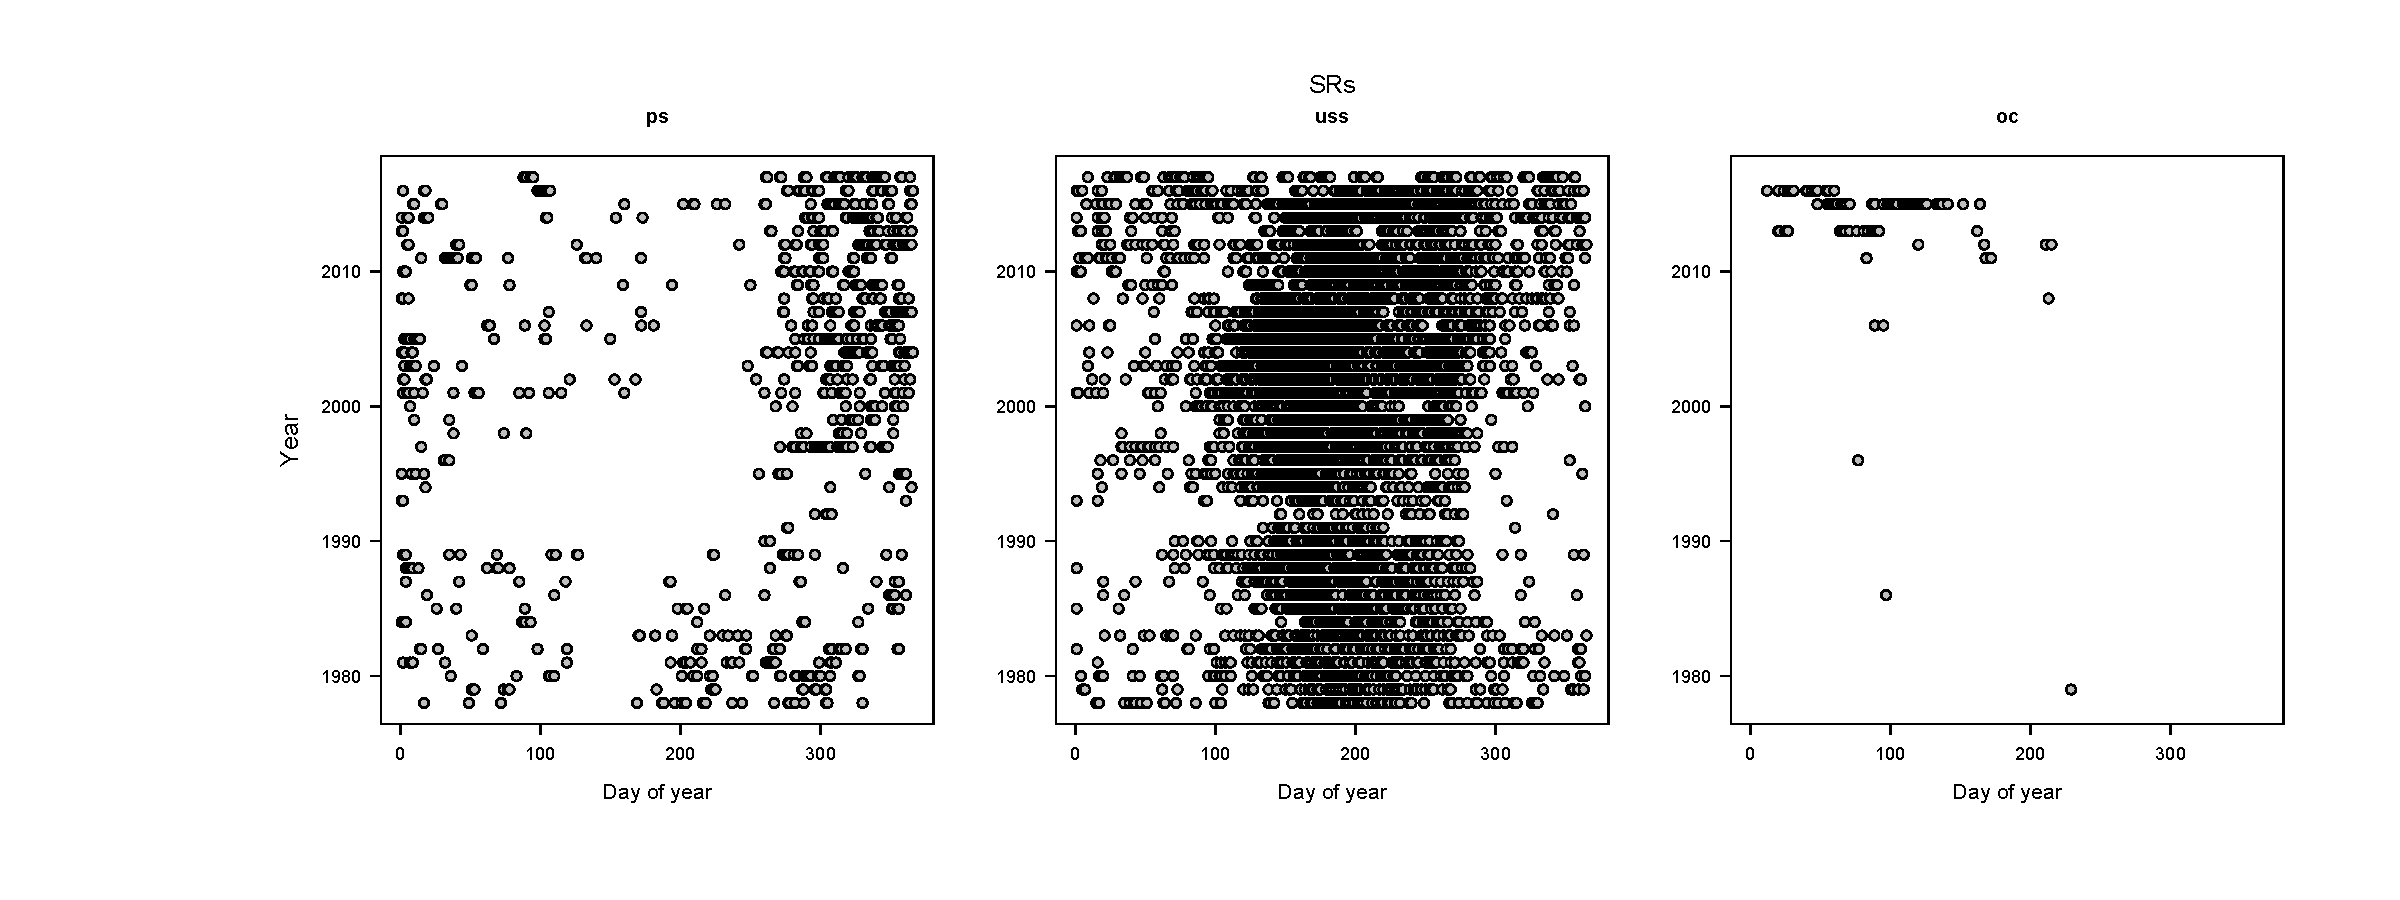
\includegraphics{/Users/ailene.ettinger/Documents/GitHub/fishphen/analyses/figures/OrcaPhenPlots/SRKW_yr_doy.pdf} 
\caption{\textbf{Southern resident killer whale activity in the Upper Salish Sea and Puget Sound varies by season}.Need to add a map of where observations are, and make this look prettier...}
 \label{fig:phenplot}
 \end{figure}
 
\begin{figure}[p]
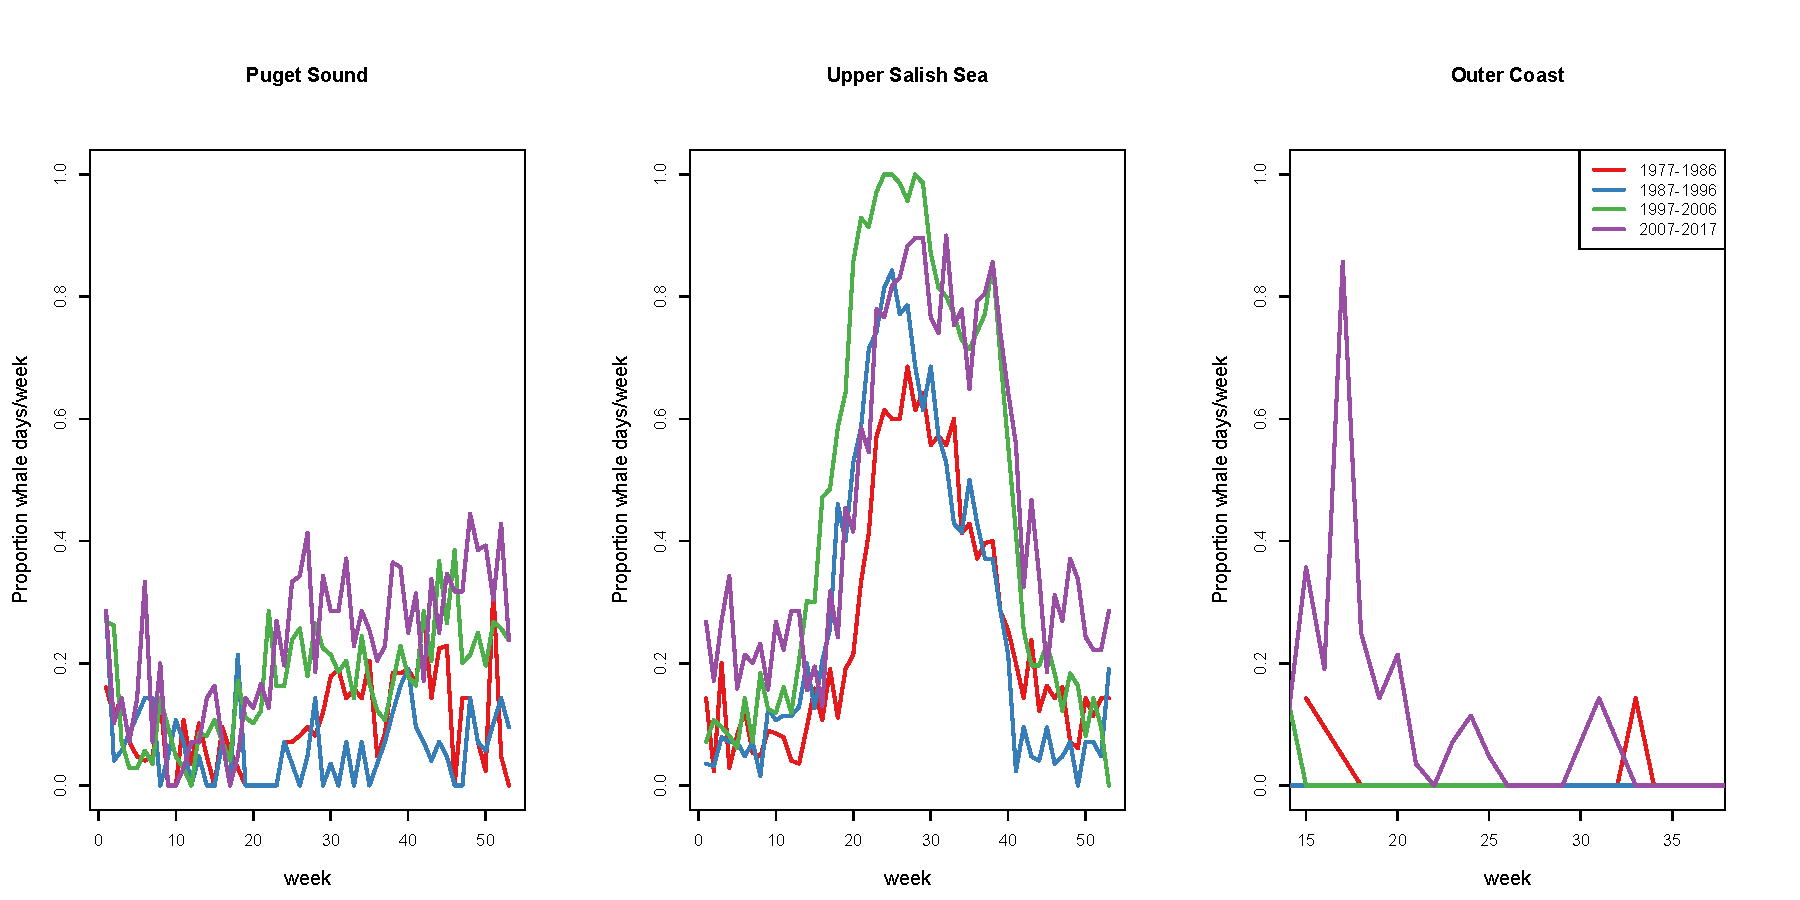
\includegraphics{/Users/ailene.ettinger/Documents/GitHub/fishphen/analyses/figures/basicplots/propwhdaysperweek.pdf} 
\caption{\textbf{Southern resident killer whale activity varies by season and region}. Lines show proportion of days per week (1 Jan= week 1) in which whales were observed in the region.}
 \label{fig:phenplot2}
 \end{figure} 
 
\begin{figure}[p]
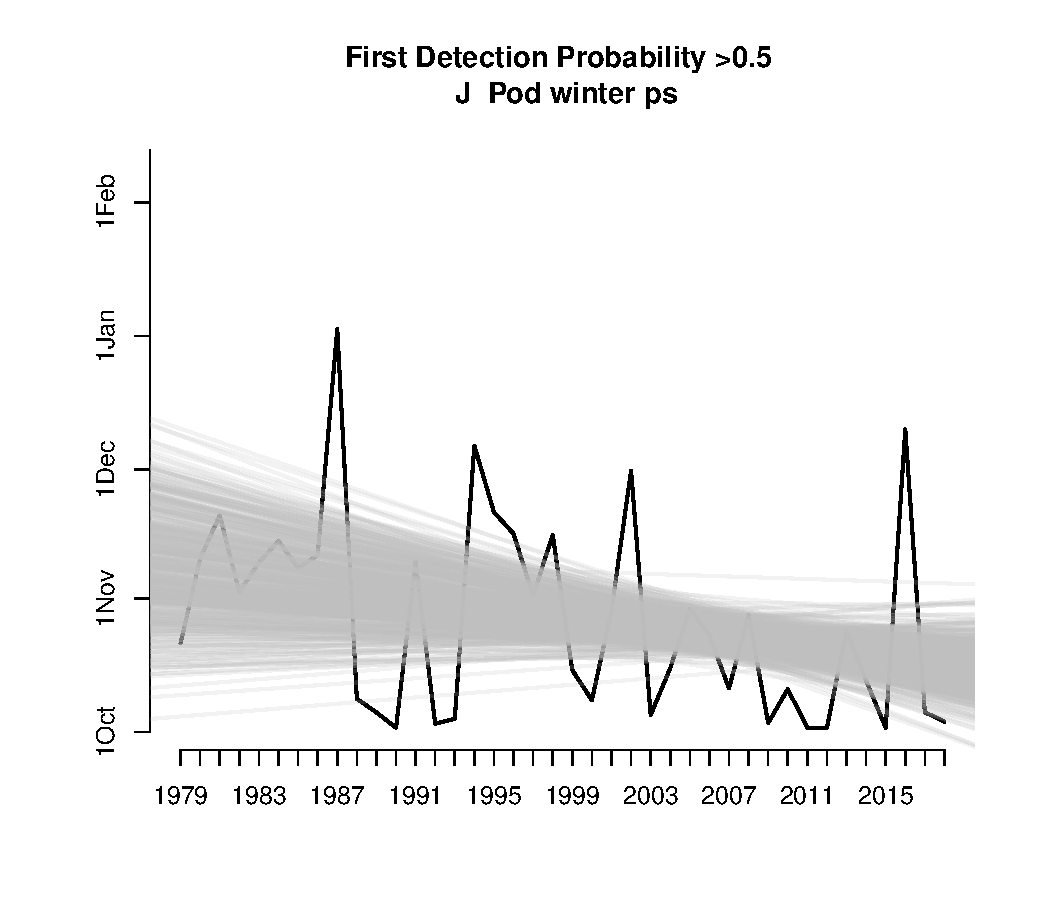
\includegraphics{/Users/ailene.ettinger/Documents/GitHub/fishphen/analyses/figures/J/orcaphen_1976_2017_PS_winter_Jfirst.pdf} 
\caption{\textbf{Trends in first- and last- observation dates for J, K, and L pod.} Make this a 6-paneled figure}
 \label{fig:trends}
 \end{figure}

\bibliography{/Users/ailene.ettinger/Documents/GitHub/fishphen/refs/noaalib.bib}
\end{document}
